Das \eigenname{QPI-SQL} Projekt hatte zum Ziel ein Fragenplugin für \eigenname{ILIAS} zu entwickeln, mit dem das \eigenname{SQL} Wissen von Testteilnehmern abgeprüft werden kann. Dieses Plugin trägt, nach den Namensschema, dass \eigenname{ILIAS} vorgibt, den Namen \eigenname{assSQLQuestion}. 
Während dieses Kapitel nicht den Umfang hat, um jedes Detail der internen Struktur von \eigenname{assSQLQuestion} näher zu erläutern, konzentriert es sich auf die dort zu findenden Besonderheiten. Dabei wird auf der einen Seite erläutert, wie der \eigenname{Javascript} Code aufgebaut ist (s. Kapitel \ref{sec:javascript}). Auf der anderen Seite wird die Besonderheit der GUI Klassen von \eigenname{assSQLQuestion} näher aufgeschlüsselt (s. Kapitel \ref{sec:gui-klassen}).

\section{Javascript}
\label{sec:javascript}

Die Struktur des \eigenname{Javascript} Codes in \eigenname{assSQLQuestion} ist dahingehend besonders, dass zum einen nicht alle \eigenname{ILIAS} Fragenplugins \eigenname{Javascript} für ihre Zwecke nutzen - siehe beispielsweise \eigenname{assExampleQuestion}. Aber auch weil der \eigenname{Javascript} Code, bei dem aus dem \eigenname{QPI-SQL} Projekt entstandenen Plugin, besondere Aufgaben zu erfüllen hat. Daraus resultieren auch besondere Klassen.

Auf der einen Seite stehen hier die sogenannten \eigenname{ExecutionInputs} und \eigenname{ExecutionOutputs}. Dies sind Javascript Klassen, die implementiert wurden, um das Einlesen von Daten aus \eigenname{HTML} Elementen, so wie die Ausgabe in selbige, von der eigentlichen Javascript Logik zu trennen. 

Auf der anderen Seite gibt es die Klassen, die die gesamte Ausführung von \eigenname{SQL} managen. \eigenname{SQLRun} übergibt die jeweilige benötige \eigenname{SQL}-Sequenz an einen \eigenname{SQL.js} Worker-Thread, während \eigenname{SQLResult} einen Datenwrapper für ein einzelnes Ergebnis einer Ausführung darstellt.

\section{GUI Klassen}
\label{sec:gui-klassen}

Im Gegensatz zu \eigenname{assExampleQuestion} und \eigenname{assCodeQuestion}, die nahezu ihre ganze GUI Logik in einer Klasse (\eigenname{assExampleQuestionGUI} bzw. \eigenname{assCodeQuestionGUI})  untergebracht haben, stellte sich bei der Entwicklung von \eigenname{assSQLQuestion} schnell heraus, dass dieses Vorgehen zu einer gigantischen und kaum zu pflegenden Klasse führen würde. Um dies zu verhindern, musste die Logik auf mehrere, logisch aufgeteilte, Klassen verteilt werden. Dies sind die sogenannten \eigenname{GUIAreas}. 

Die Idee hinter der Struktur dieser Klassen basiert darauf, dass sich die GUI von Fragenplugins in \eigenname{ILIAS} in drei Szenen einteilt. Eine Szene beschreibt die GUI beim Anlegen und Bearbeiten einer Szene, eine Zweite beschreibt die Fragenvorschau, so wie die Anzeige der eigentlichen Frage in einem Test, und eine Dritte betrifft die Anzeige der Lösung.

Dabei besitzt \eigenname{assSQLQuestion} vier GUI Bereiche, die sich in jeder dieser Szenen wiederholen. Einmal den Bereich der die Frage wiedergibt, den Bereich der die \eigenname{SQL}-Sequenzen enthält, den Bereich der die Ausgabe beinhaltet und den Bereich der die Metriken umschließt. In Abbildung \ref{fig:gui-bereiche} ist dies gut zu sehen:

    \begin{figure}[H]
        \begin{center}
            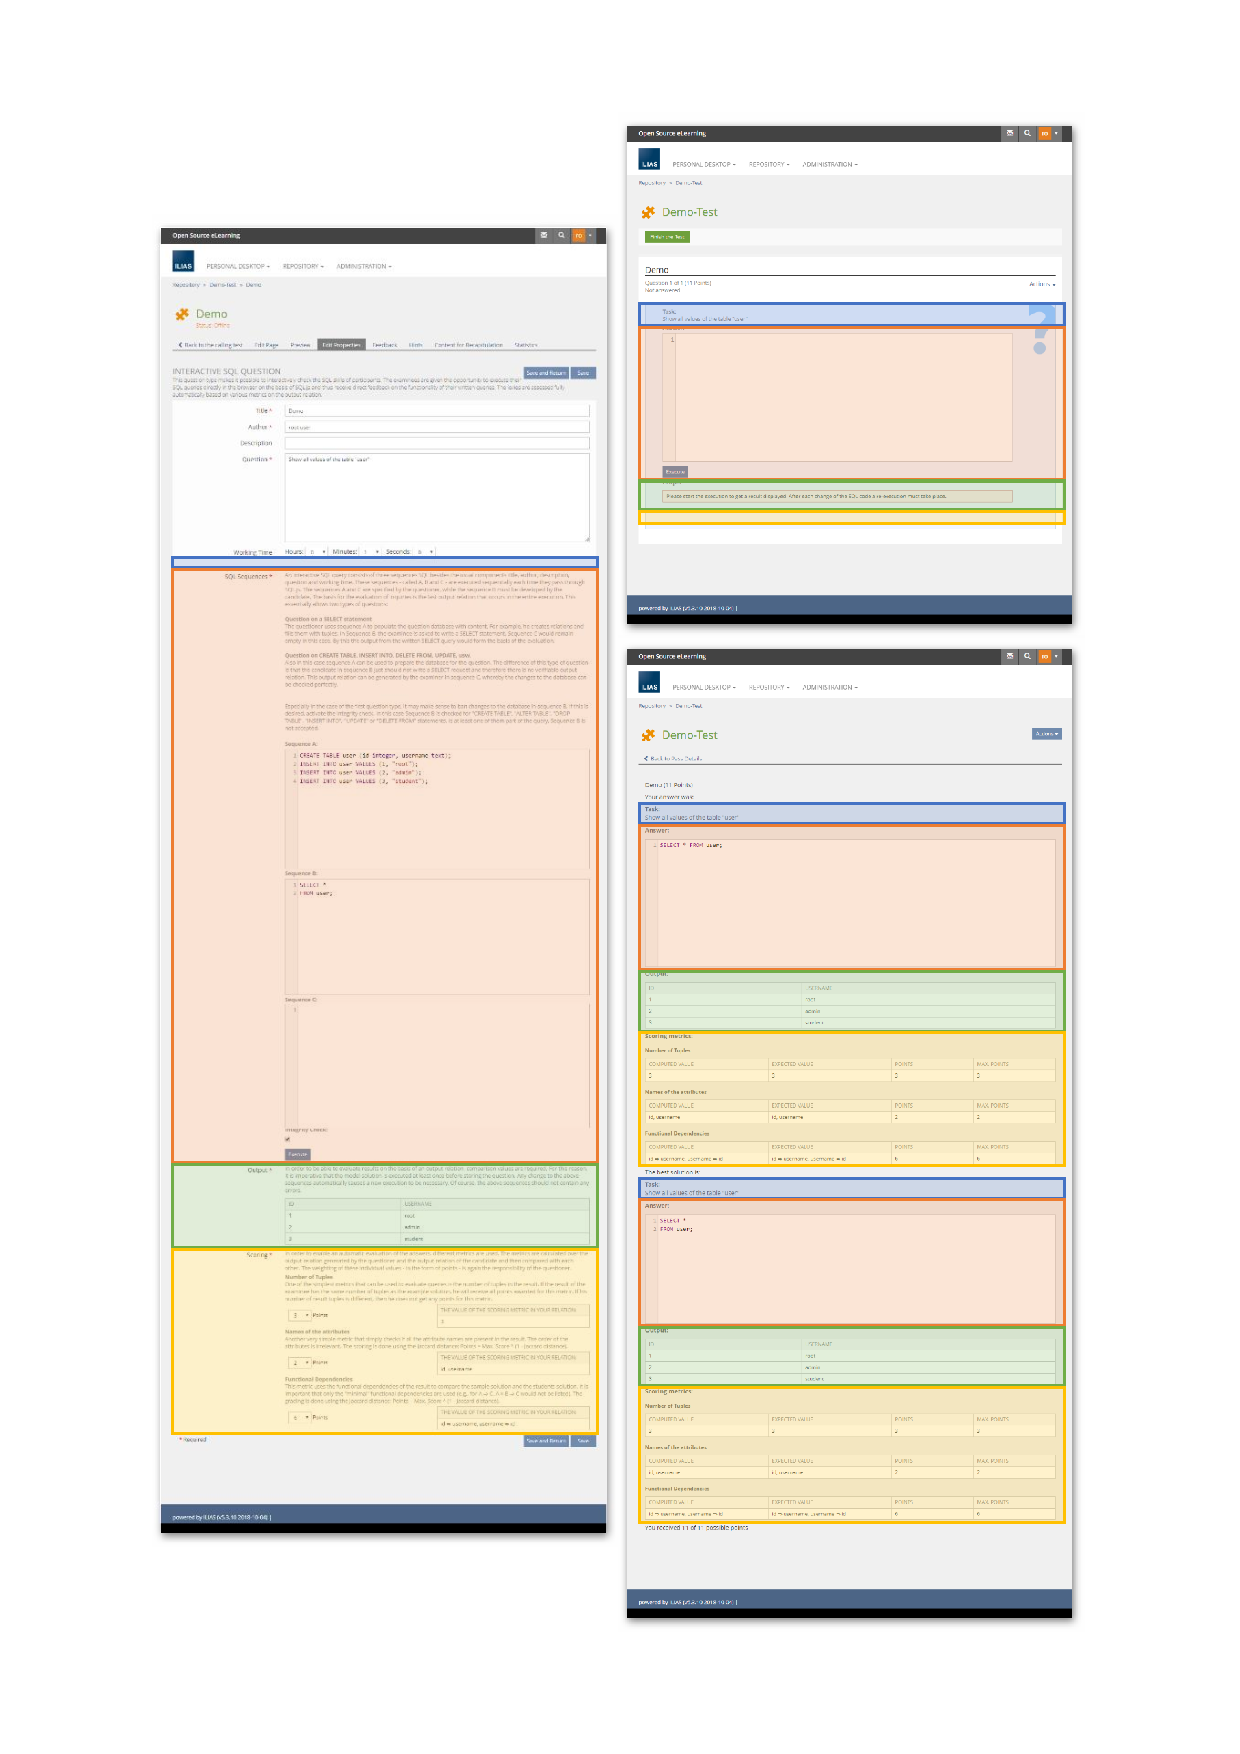
\includegraphics[page=1, width=0.3\paperwidth, trim=4 4 4 4, clip]{fig/GUIAreas.pdf} 
            \caption{GUI-Bereiche von \eigenname{assSQLQuestion}}
            \label{fig:gui-bereiche}
        \end{center}
    \end{figure}
    
Jeder dieser Bereiche bildet nun in der internen Struktur eine eigene \eigenname{GUIArea}, welche von \eigenname{assSQLQuestionGUI} nur noch aufgerufen wird, und seine eigene Logik implementiert. 




